\documentclass[10pt,a4paper]{ULBreport}
\usepackage[utf8]{inputenc}
\sceau{pic/official_logos/sceauULB.png}
\graphicspath{ {./pic/} }
\usepackage{multirow}
\usepackage{listings}
\usepackage{color} 
\usepackage{setspace} 
\usepackage{amsmath}
\usepackage{hyperref}
\usepackage{pdfpages}
\usepackage{biblatex}
\usepackage{floatrow}
\usepackage{subcaption} 
\usepackage{siunitx}
\usepackage[many]{tcolorbox}
\usepackage{multirow}
\usepackage{listings}
\usepackage[dvipsnames]{xcolor}
\usepackage{fancyvrb}

\usepackage{xstring}
\usepackage{etoolbox}

% Colors



\begin{document} 


	\titleULB{
	title={DVB-C project},
    studies={M1-IRELE},
    course ={ELEC-H401 Modulation and coding},
    author={\textit{Authors :} \\ Arico Amaury \\ Colot Emmeran },
    date={\textbf{Academic year :} \\ 2024 - 2025},
    teacher={\textit{Professor : } \\ Horlin François},
    logo={pic/official_logos/logos.jpg},
    manyAuthor
	}

%\listoftables % ToC for tables

%\listoffigures % ToC for figures

\setcounter{secnumdepth}{-1}

\chapter{Introduction}

This report aims to complete the code that simulates a DVB-C transmission chain in matlab. It answers the questions asked after each major step of the project and analyses the results of the simulation.

\vspace{2cm}

\begin{figure}[H]
    \centering
    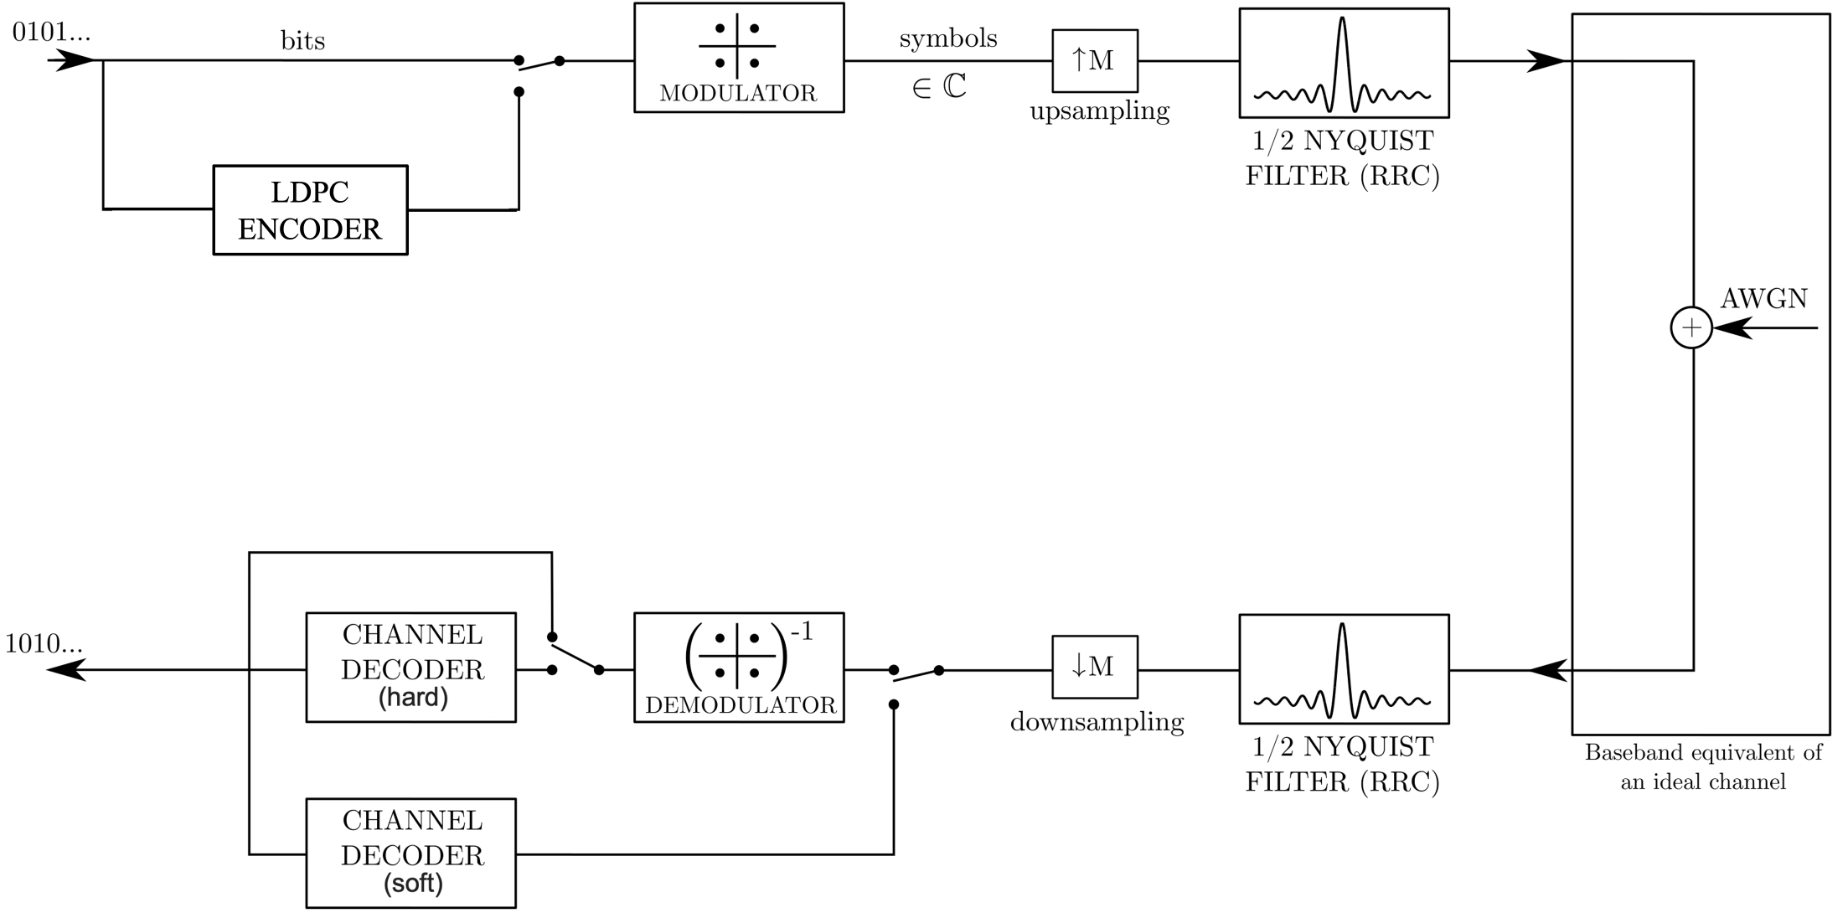
\includegraphics[width=0.9\linewidth]{blockDiagram.png}
    \caption{DVB-C transmission chain}
    \label{fig:blockDiagram}
\end{figure}


%\printglossary

%\printglossary[type=\acronymtype]

%Bibliography
%\nocite{*}
%\printbibliography[type=article,title=Articles]

\end{document}	
